\documentclass[11pt]{article}
\usepackage[a4paper,margin=2.4cm]{geometry}

\usepackage{booktabs,graphicx,amsmath,hyperref,xcolor}
\hypersetup{colorlinks,linkcolor=blue!50!black,citecolor=blue!50!black,urlcolor=blue!50!black}
\usepackage[numbers,sort&compress]{natbib}

\title{Does Attack-Path Awareness Help Prioritise Cloud Security Findings?\\
\large An Empirical Study on 600 Synthetic Architectures}
\author{Mithil Nagabathula\\University of East London\\\texttt{mithilnishu2000@gmail.com}}
\date{October 2026}

\begin{document}
\maketitle

\begin{abstract}
Threat-modelling-as-code tools flag dozens of design weaknesses in a cloud architecture, and teams fix them a few at a time.
The order matters, yet tools usually rank findings by a fixed rule severity or by a hand-built risk score.
We ask whether attack-path awareness ranks them better.
Using the open-source SentinelCloud engine unmodified, we generate 600 synthetic architectures, produce \(9.7\) findings each on average,
and compare five orderings against an independent noisy-OR attacker model that measures the share of achievable expected-loss reduction
realised after each fix.
Three results stand out.
First, a plain severity ordering (0.625 of the achievable reduction, averaged over the first five fixes) beat both the tool's own risk model (0.475)
and an attack-path ordering (0.575), in every one of 16 sensitivity settings; attack paths helped only with the very first fix.
Second, the risk model's weakness has a specific cause: its likelihood term ignores data stores that are directly reachable from the internet,
so it never chose to close public network access first. Correcting that term lifted it to 0.726.
Third, a greedy ordering guided by a probabilistic model whose parameters were each perturbed by up to \(\pm50\%\) reached 0.795, close to the
0.811 obtained with the true parameters.
The results are from a synthetic corpus and a model-based ground truth, so they show what to test on real estates rather than settle the question;
code and data are released.
\end{abstract}

\section{Introduction}
Design-time security review is moving into code. Threat-modelling-as-code tools read an architecture description, apply rules,
and fail a pipeline when a rule fires \cite{shostack2014threat}. A typical design produces many findings: over-broad identities,
unauthenticated internal flows, public data stores, flat network zones. Engineering time is limited, so the practical question is
\emph{which findings to fix first}.

Three kinds of answer are common. A \emph{severity} ordering uses a fixed label per rule, much as CVSS base scores do for vulnerabilities
\cite{first2019cvss}. A \emph{risk} ordering multiplies the impact of the assets a finding touches by how exposed they are.
An \emph{attack-path} ordering, drawing on the attack-graph literature \cite{sheyner2002attackgraphs,ou2005mulval}, prefers findings that
sit on feasible routes from the internet to sensitive data. The intuition behind the last is strong, but is it borne out?

This paper tests the three orderings on the same findings, produced by the same unmodified engine, against an independent measure of
how much each fix reduces expected loss. Our contributions are:
\begin{itemize}
  \item a reproducible benchmark: a generator of 600 cloud architectures in SentinelCloud's schema \cite{sentinelcloud}, a remediation
        operator per rule, and a noisy-OR attacker model used only for evaluation;
  \item evidence that, in this setting, rule severity outperforms both a risk score and attack-path ordering, and a diagnosis of why;
  \item evidence that a cheap probabilistic model used \emph{for ordering} is robust to large errors in its parameters.
\end{itemize}

\section{Related work}
Attack graphs model how an attacker chains weaknesses \cite{sheyner2002attackgraphs,ou2005mulval}. Probabilistic variants attach
success probabilities to edges and combine them into a metric \cite{wang2008probabilistic,homer2013aggregating}; our evaluation
model follows this tradition with a noisy-OR fixed point. Hardening work asks which set of changes breaks all paths at least cost
\cite{noel2003hardening,dewri2007optimal}. Vulnerability prioritisation has moved from static severity towards predicted exploitation
\cite{jacobs2021epss}. We differ in focus: we study design-level findings from a threat-modelling tool rather than host vulnerabilities,
and we compare the ranking heuristics practitioners actually get from such tools.

\section{Method}
\subsection{Engine and strategies}
SentinelCloud \cite{sentinelcloud} applies ten rules to an architecture description (assets, flows, trust boundaries, identity bindings,
logging). We use its rule engine, risk model and attack-path simulator without modification, and compare:
\begin{description}
  \item[Severity] the engine's fixed rule severity (CRITICAL, HIGH, MEDIUM), ties broken by engine order, as a CI gate would see them.
  \item[Risk] SentinelCloud's risk model: impact (sensitivity of touched assets, including one outgoing hop) times likelihood
        (structural exposure via internet-facing flows).
  \item[Path] findings ranked by the sensitivity-weighted number of high-feasibility attack chains (from the simulator) they lie on,
        then by severity.
  \item[Random] the mean of 20 random orderings (lower reference).
  \item[Oracle] at each step, the fix that most reduces expected loss under the evaluation model (upper reference).
\end{description}
We add two variants in Section~\ref{sec:ext}: an exposure-corrected risk model, and a greedy ordering using a deliberately misspecified
attacker model.

\subsection{Corpus}
The generator draws an architecture of a given size (small, medium or large: 2--4, 5--8 or 9--14 services and 1--3, 3--5 or 5--9 data
stores) with a latent \emph{hardening} level in \([0,1]\) that lowers the probability of every weakness. Architectures with fewer than three
findings are discarded. The corpus has 600 architectures (200 per size), with on average 13.8 assets, 17.1 flows and 9.7 findings
(range 3--32).

\subsection{Evaluation model}
Ground truth is an expected-loss model that none of the ranking strategies use. Each asset \(v\) has a compromise probability \(P_v\).
Internet-facing gateways and publicly reachable data stores receive direct probabilities; flows, flat trust boundaries and identity
bindings form attack edges with success probabilities \(p_{uv}\) (for example 0.1 for an authenticated hop, 0.6 for an unauthenticated
one, 0.8 for a workload identity with subscription-wide scope). Probabilities are propagated to a fixed point with noisy-OR,
\[
  P_v = 1 - (1 - d_v)\prod_{(u,v)} \bigl(1 - P_u\, p_{uv}\bigr),
\]
and loss is \(\mathcal{L} = \sum_{s} w_s P_s\) over sensitive assets, with \(w_s \in \{1,2,3,4\}\) by sensitivity, multiplied by 1.5 when
the store is unencrypted. Logging dampens edge probabilities by 15\%. Each rule has a remediation operator that applies the fix its own
mitigation text describes (for example, splitting a flat zone, disabling public access, or scoping an identity).

For an architecture with initial loss \(\mathcal{L}_0\) and loss \(\mathcal{L}_{\text{all}}\) after fixing every finding, the score after
\(k\) fixes is the share of achievable reduction \(r_k = (\mathcal{L}_0 - \mathcal{L}_k)/(\mathcal{L}_0 - \mathcal{L}_{\text{all}})\).
We report \(r_1\), \(r_3\) and the mean of \(r_1,\dots,r_5\) (the area under the first five fixes). Strategies are compared with paired
two-sided Wilcoxon signed-rank tests \cite{wilcoxon1945} over architectures.

\section{Results}
\begin{table*}[t]
\centering
\caption{Share of the achievable loss reduction realised by each prioritisation strategy across 600 synthetic architectures (mean $\pm$ 95\% CI). The last column is the mean paired difference in the 1--5 mean against rule severity, with a two-sided Wilcoxon signed-rank test.}
\label{tab:main}
\small
\setlength{\tabcolsep}{4pt}
\begin{tabular}{lrrrr}
\toprule
Strategy & After 1 fix & After 3 fixes & Mean over 1--5 & vs.~severity \\
\midrule
Random order & 0.175 $\pm$ 0.010 & 0.488 $\pm$ 0.021 & 0.437 $\pm$ 0.016 & -0.188 ($p<0.001$) \\
Risk model (original) & 0.265 $\pm$ 0.021 & 0.522 $\pm$ 0.028 & 0.475 $\pm$ 0.021 & -0.151 ($p<0.001$) \\
Attack-path aware & 0.319 $\pm$ 0.022 & 0.628 $\pm$ 0.025 & 0.575 $\pm$ 0.019 & -0.050 ($p<0.001$) \\
Rule severity & 0.292 $\pm$ 0.025 & 0.707 $\pm$ 0.024 & 0.625 $\pm$ 0.019 & -- \\
Risk model (exposure-corrected) & 0.423 $\pm$ 0.024 & 0.801 $\pm$ 0.019 & 0.726 $\pm$ 0.016 & +0.101 ($p<0.001$) \\
Model-guided, $\pm$50\% misspecified & 0.525 $\pm$ 0.020 & 0.860 $\pm$ 0.013 & 0.795 $\pm$ 0.012 & +0.170 ($p<0.001$) \\
Model-guided, true parameters & 0.554 $\pm$ 0.019 & 0.873 $\pm$ 0.012 & 0.811 $\pm$ 0.011 & +0.186 ($p<0.001$) \\
\bottomrule
\end{tabular}
\end{table*}


\paragraph{Severity beats both the risk score and attack paths.}
Table~\ref{tab:main} shows the main result. Over the first five fixes, severity realised 0.625 of the achievable reduction, the attack-path
ordering 0.575 and the risk model 0.475, against 0.437 for random order and 0.811 for the oracle. Path-aware ordering did win on the very first
fix (0.319 against 0.292; mean paired difference \(+0.027\), \(p<0.001\)), but fell behind from the second fix on. The advantage of severity
held for every architecture size (Figure~\ref{fig:size}) and grew as hardening fell: the gap between path and severity correlated
negatively with hardening (Spearman \(\rho=-0.16\), \(p<0.001\)).

\begin{figure}[t]
  \centering
  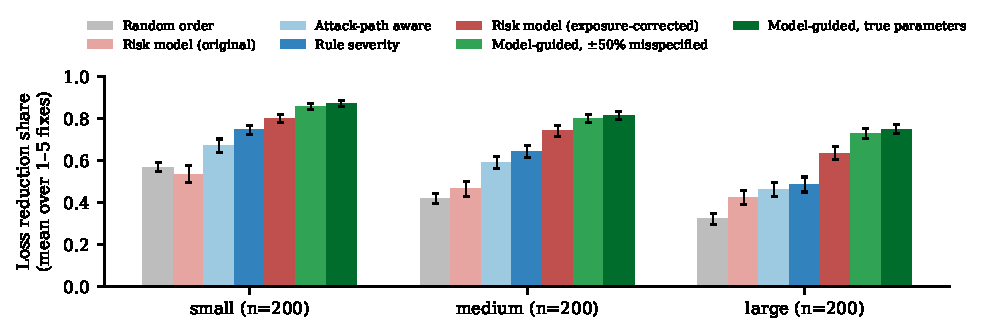
\includegraphics[width=\linewidth]{figures/by_size.pdf}
  \caption{Mean share of achievable loss reduction over the first five fixes, by architecture size (error bars: 95\% CI).}
  \label{fig:size}
\end{figure}

\paragraph{Why.}
Table~\ref{tab:rules} lists, for each rule, the value of fixing one of its findings alone and how often each strategy picked that rule first.
The two most valuable fixes are splitting a flat zone that holds both compute and data (NET-SEGMENT-01, 0.41) and disabling public
network access on a data store (NET-PUBLIC-01, 0.31). The oracle chose NET-PUBLIC-01 first in a third of architectures; the risk model
\emph{never} did. Its likelihood term scores exposure only through flows from internet-facing assets, so a database open to the internet
with no flow from a gateway looks unexposed. The path ordering found NET-SEGMENT-01 (first in 206 architectures) but over-weighted
findings that happen to lie on many chains, such as missing WAFs and logging, whose individual value is modest. Severity favours
IAM-BROAD-01, which is moderately valuable and very common, and that is enough to make it a robust default.

\begin{table}[t]
\centering
\caption{Value of fixing each rule's findings on their own (share of the achievable loss reduction, averaged over findings), and how often each strategy chooses that rule as its first fix.}
\label{tab:rules}
\small
\setlength{\tabcolsep}{4pt}
\begin{tabular}{lrrrrrr}
\toprule
Rule & Findings & Mean value of fixing alone & Sev. & Risk & Path & Oracle \\
\midrule
NET-SEGMENT-01 & 228 & 0.406 & 31 & 133 & 206 & 147 \\
NET-PUBLIC-01 & 569 & 0.312 & 111 & 0 & 40 & 200 \\
NET-PUBLIC-02 & 157 & 0.266 & 23 & 1 & 11 & 54 \\
NET-WAF-01 & 348 & 0.216 & 0 & 37 & 91 & 50 \\
LOG-001 & 161 & 0.156 & 3 & 49 & 73 & 2 \\
IAM-BROAD-01 & 677 & 0.130 & 385 & 205 & 67 & 68 \\
DATA-ENC-01 & 491 & 0.104 & 22 & 0 & 18 & 6 \\
AUTHN-FLOW-01 & 2231 & 0.064 & 14 & 115 & 49 & 56 \\
IAM-MISSING-01 & 535 & 0.059 & 5 & 34 & 20 & 17 \\
IAM-BROAD-02 & 433 & 0.015 & 6 & 26 & 25 & 0 \\
\bottomrule
\end{tabular}
\end{table}


\subsection{Extensions}\label{sec:ext}
\paragraph{Correcting the risk model.} Adding the two cases the likelihood term misses (data stores with public network or blob access,
scored as maximally exposed) raised the risk model from 0.475 to 0.726, above severity by \(+0.101\) (\(p<0.001\); better in 77\% of
architectures).

\paragraph{Model-guided ordering under misspecification.} We ran the oracle's greedy procedure with an attacker model whose every parameter
was independently multiplied by a factor drawn from \(U(0.5, 1.5)\), averaging three draws per architecture. It reached 0.795, against 0.811
with the true parameters, and beat severity in 94\% of architectures. The ordering is far less sensitive to the parameter values than the
loss itself, because it depends mostly on the \emph{structure} of the attack graph.

\paragraph{Sensitivity of the main result.} Halving or raising each of eight attacker-model parameters by 50\% (Table~\ref{tab:sens},
150 architectures per setting) never changed the ranking: severity beat both path and risk in all 16 settings, with severity in
\([0.53, 0.61]\), path in \([0.47, 0.56]\) and risk in \([0.41, 0.51]\).

\begin{table}[t]
\centering
\caption{Sensitivity analysis: mean loss-reduction share over 1--5 fixes when one attacker-model parameter is halved or raised by 50\% (150 architectures each).}
\label{tab:sens}
\small
\setlength{\tabcolsep}{4pt}
\begin{tabular}{llrrrr}
\toprule
Parameter & Change & Severity & Risk & Path & Oracle \\
\midrule
flat-zone lateral move & $\times$0.5 & 0.581 & 0.431 & 0.494 & 0.774 \\
flat-zone lateral move & $\times$1.5 & 0.567 & 0.463 & 0.530 & 0.789 \\
authenticated hop & $\times$0.5 & 0.574 & 0.451 & 0.513 & 0.805 \\
authenticated hop & $\times$1.5 & 0.570 & 0.449 & 0.520 & 0.766 \\
unauthenticated hop & $\times$0.5 & 0.614 & 0.411 & 0.501 & 0.813 \\
unauthenticated hop & $\times$1.5 & 0.532 & 0.467 & 0.516 & 0.760 \\
gateway without WAF & $\times$0.5 & 0.594 & 0.424 & 0.469 & 0.799 \\
gateway without WAF & $\times$1.5 & 0.558 & 0.461 & 0.537 & 0.785 \\
missing identity & $\times$0.5 & 0.584 & 0.451 & 0.519 & 0.792 \\
missing identity & $\times$1.5 & 0.563 & 0.449 & 0.514 & 0.775 \\
subscription-wide identity & $\times$0.5 & 0.546 & 0.431 & 0.517 & 0.793 \\
subscription-wide identity & $\times$1.5 & 0.580 & 0.456 & 0.516 & 0.781 \\
public data store & $\times$0.5 & 0.563 & 0.509 & 0.557 & 0.784 \\
public data store & $\times$1.5 & 0.577 & 0.420 & 0.495 & 0.785 \\
unencrypted impact & $\times$0.5 & 0.561 & 0.453 & 0.501 & 0.790 \\
unencrypted impact & $\times$1.5 & 0.578 & 0.451 & 0.524 & 0.785 \\
\bottomrule
\end{tabular}
\end{table}


\section{Discussion and limitations}
The tempting conclusion, that attack paths are the right lens for design findings, did not hold in this study, but a related one did:
reasoning about the attack graph \emph{probabilistically and greedily}, rather than counting chains, was the best practical strategy and
tolerated large parameter errors. Counting chains rewards findings that are on many paths without asking whether fixing them actually
breaks those paths. A second lesson is mundane but useful: a single blind spot in a likelihood function can make a risk score worse than
the severity labels it was meant to improve, so risk scores need testing against an independent measure.

The limitations are substantial. (1) The corpus is synthetic; real architectures may have different weakness correlations. (2) The ground
truth is a model, and the oracle and greedy strategies share its structure, which favours them; the misspecification experiment addresses
parameter error but not structural error. (3) Remediation operators are idealised: every fix is applied fully and at equal cost.
(4) All strategies use one engine's ten rules. (5) The study's author also wrote SentinelCloud; the engine was used without modification,
and the code is released so that others can check the results. A natural next step is to rank findings from real, anonymised
architecture reviews and compare with incident or red-team data.

\section{Conclusion}
On 600 synthetic cloud architectures, fixed rule severity outperformed both a risk score and attack-path ordering for prioritising design
findings, while a greedy ordering driven by an approximate probabilistic attacker model came close to optimal even with parameters off by
up to 50\%. Tools that rank design findings should test their scores against an independent loss model; when they can, they should use
probabilistic reasoning over the attack graph rather than counting paths.

\paragraph{Reproducibility.} Code, the generated corpus and all result files will be released at
\url{https://github.com/mithil2k2000-tech/attack-path-prioritisation}.

\paragraph{Use of AI tools.} An AI assistant (Claude, Anthropic) helped write experiment code and draft text. The author designed the study
questions, reviewed the code and results, and takes responsibility for the content.

\bibliographystyle{plainnat}
\bibliography{refs}
\end{document}
